\documentclass[utf8x, 12pt]{G7-32}

% Настройки стиля ГОСТ 7-32
% Для начала определяем, хотим мы или нет, чтобы рисунки и таблицы нумеровались в пределах раздела, или нам нужна сквозная нумерация.
\EqInChapter % формулы будут нумероваться в пределах раздела
\TableInChapter % таблицы будут нумероваться в пределах раздела
\PicInChapter % рисунки будут нумероваться в пределах раздела
\usepackage{slashbox}

\usepackage[table,xcdraw]{xcolor}

% Добавляем гипертекстовое оглавление в PDF
\usepackage[
bookmarks=true, colorlinks=true, unicode=true,
urlcolor=black,linkcolor=black, anchorcolor=black,
citecolor=black, menucolor=black, filecolor=black,
]{hyperref}

% Изменение начертания шрифта --- после чего выглядит таймсоподобно.
% \usepackage{cyrtimespatched}

% графика
\usepackage{graphicx}
\graphicspath{ {./img/} }

% отделять первую строку раздела абзацным отступом
\usepackage{indentfirst} 

% Пакет Tikz
\usepackage{tikz}
\usetikzlibrary{arrows,positioning,shadows}

% Произвольная нумерация списков.
\usepackage{enumerate}

% ячейки в несколько строчек
\usepackage{multirow}

% itemize внутри tabular
\usepackage{paralist,array}

% объявляем новую команду для переноса строки внутри ячейки таблицы
\newcommand{\specialcell}[2][c]{%
	\begin{tabular}[#1]{@{}c@{}}#2\end{tabular}}

\usepackage{tikz}
\usepackage{pgfplots}
\usepackage{pdfpages}
\usepackage{caption}
% \captionsetup[table]{position=top}
% Листинги

\usepackage{listings}
\usepackage{caption}

\usepackage{courier}
\usepackage{wrapfig}

\usepackage{xcolor}
\captionsetup[lstlisting]{singlelinecheck=off, justification=raggedright}


\definecolor{codegreen}{rgb}{0,0.6,0}
\definecolor{codegray}{rgb}{0.5,0.5,0.5}
\definecolor{codepurple}{rgb}{0.58,0,0.82}
\definecolor{backcolour}{rgb}{0.95,0.95,0.92}


% Значения по умолчанию
\lstset{
  % подсветка синтаксиса
  backgroundcolor=\color{backcolour},   
  commentstyle=\color{codegreen},
  keywordstyle=\color{magenta},
  numberstyle=\tiny\color{codegray},
  stringstyle=\color{codepurple},
  basicstyle= \footnotesize,
  breakatwhitespace=true,% разрыв строк только на whitespacce
  breaklines=true,       % переносить длинные строки
%   captionpos=b,          % подписи снизу -- вроде не надо
  inputencoding=koi8-r,
  numbers=left,          % нумерация слева
  numberstyle=\footnotesize,
  showspaces=false,      % показывать пробелы подчеркиваниями -- идиотизм 70-х годов
  showstringspaces=false,
  showtabs=false,        % и табы тоже
  stepnumber=1,
  tabsize=4,              % кому нужны табы по 8 символов?
  frame=single,
  escapeinside={(*}{*)}, %выделение
  literate={а}{{\selectfont\char224}}1
  {б}{{\selectfont\char225}}1
  {в}{{\selectfont\char226}}1
  {г}{{\selectfont\char227}}1
  {д}{{\selectfont\char228}}1
  {е}{{\selectfont\char229}}1
  {ё}{{\"e}}1
  {ж}{{\selectfont\char230}}1
  {з}{{\selectfont\char231}}1
  {и}{{\selectfont\char232}}1
  {й}{{\selectfont\char233}}1
  {к}{{\selectfont\char234}}1
  {л}{{\selectfont\char235}}1
  {м}{{\selectfont\char236}}1
  {н}{{\selectfont\char237}}1
  {о}{{\selectfont\char238}}1
  {п}{{\selectfont\char239}}1
  {р}{{\selectfont\char240}}1
  {с}{{\selectfont\char241}}1
  {т}{{\selectfont\char242}}1
  {у}{{\selectfont\char243}}1
  {ф}{{\selectfont\char244}}1
  {х}{{\selectfont\char245}}1
  {ц}{{\selectfont\char246}}1
  {ч}{{\selectfont\char247}}1
  {ш}{{\selectfont\char248}}1
  {щ}{{\selectfont\char249}}1
  {ъ}{{\selectfont\char250}}1
  {ы}{{\selectfont\char251}}1
  {ь}{{\selectfont\char252}}1
  {э}{{\selectfont\char253}}1
  {ю}{{\selectfont\char254}}1
  {я}{{\selectfont\char255}}1
  {А}{{\selectfont\char192}}1
  {Б}{{\selectfont\char193}}1
  {В}{{\selectfont\char194}}1
  {Г}{{\selectfont\char195}}1
  {Д}{{\selectfont\char196}}1
  {Е}{{\selectfont\char197}}1
  {Ё}{{\"E}}1
  {Ж}{{\selectfont\char198}}1
  {З}{{\selectfont\char199}}1
  {И}{{\selectfont\char200}}1
  {Й}{{\selectfont\char201}}1
  {К}{{\selectfont\char202}}1
  {Л}{{\selectfont\char203}}1
  {М}{{\selectfont\char204}}1
  {Н}{{\selectfont\char205}}1
  {О}{{\selectfont\char206}}1
  {П}{{\selectfont\char207}}1
  {Р}{{\selectfont\char208}}1
  {С}{{\selectfont\char209}}1
  {Т}{{\selectfont\char210}}1
  {У}{{\selectfont\char211}}1
  {Ф}{{\selectfont\char212}}1
  {Х}{{\selectfont\char213}}1
  {Ц}{{\selectfont\char214}}1
  {Ч}{{\selectfont\char215}}1
  {Ш}{{\selectfont\char216}}1
  {Щ}{{\selectfont\char217}}1
  {Ъ}{{\selectfont\char218}}1
  {Ы}{{\selectfont\char219}}1
  {Ь}{{\selectfont\char220}}1
  {Э}{{\selectfont\char221}}1
  {Ю}{{\selectfont\char222}}1
  {Я}{{\selectfont\char223}}1
}

\lstloadlanguages{
  C++
}

% Стиль для псевдокода: строчки обычно короткие, поэтому размер шрифта побольше
\lstdefinestyle{pseudocode}{
  basicstyle=\small,
  keywordstyle=\color{black}\bfseries\underbar,
  language=Pseudocode,
  numberstyle=\footnotesize,
  commentstyle=\footnotesize\it
}

% Стиль для обычного кода: маленький шрифт
\lstdefinestyle{realcode}{
  basicstyle=\scriptsize,
  numberstyle=\footnotesize
}

% Стиль для коротких кусков обычного кода: средний шрифт
\lstdefinestyle{simplecode}{
  basicstyle=\footnotesize,
  numberstyle=\footnotesize
}

% Стиль для BNF
\lstdefinestyle{grammar}{
  basicstyle=\footnotesize,
  numberstyle=\footnotesize,
  stringstyle=\bfseries\ttfamily,
  language=BNF
}

% Определим свой язык для написания псевдокодов на основе Python
\lstdefinelanguage[]{Pseudocode}[]{Python}{
  morekeywords={each,empty,wait,do},% ключевые слова добавлять сюда
  morecomment=[s]{\{}{\}},% комменты {а-ля Pascal} смотрятся нагляднее
  literate=% а сюда добавлять операторы, которые хотите отображать как мат. символы
    {->}{\ensuremath{$\rightarrow$}~}2%
    {<-}{\ensuremath{$\leftarrow$}~}2%
    {:=}{\ensuremath{$\leftarrow$}~}2%
    {<--}{\ensuremath{$\Longleftarrow$}~}2%
}[keywords,comments]

% Свой язык для задания грамматик в BNF
\lstdefinelanguage[]{BNF}[]{}{
  morekeywords={},
  morecomment=[s]{@}{@},
  morestring=[b]",%
  literate=%
    {->}{\ensuremath{$\rightarrow$}~}2%
    {*}{\ensuremath{$^*$}~}2%
    {+}{\ensuremath{$^+$}~}2%
    {|}{\ensuremath{$|$}~}2%
}[keywords,comments,strings]

% Подписи к листингам на русском языке.
\renewcommand\lstlistingname{\cyr\CYRL\cyri\cyrs\cyrt\cyri\cyrn\cyrg}
\renewcommand\lstlistlistingname{\cyr\CYRL\cyri\cyrs\cyrt\cyri\cyrn\cyrg\cyri}



\begin{document}

\frontmatter % выключает нумерацию ВСЕГО; здесь начинаются ненумерованные главы: реферат, введение, глоссарий, сокращения и прочее.

\begin{table}[ht]
	\centering
	\begin{tabular}{|c|p{400pt}|} 
	\hline
		\begin{tabular}[c]{@{}c@{}} 
\includegraphics[scale=0.37]{EmblemBMSTU} \\\end{tabular} &
		\footnotesize\begin{tabular}[c]{@{}c@{}}\textbf{Министерство~науки~и~высшего~образования~Российской~Федерации}\\\textbf{Федеральное~государственное~бюджетное~образовательное~учреждение}\\\textbf{~высшего~образования}\\\textbf{«Московский~государственный~технический~университет}\\\textbf{имени~Н.Э.~Баумана}\\\textbf{(национальный~исследовательский~университет)»}\\\textbf{(МГТУ~им.~Н.Э.~Баумана)}\\\end{tabular}  \\
	\hline
	\end{tabular}
\end{table}
\noindent\rule{\textwidth}{4pt}
\noindent\rule[14pt]{\textwidth}{1pt}
\hfill 
\noindent
\makebox{ФАКУЛЬТЕТ~}%
\makebox[\textwidth][l]{\underline{~~~~«Информатика и системы управления»~~~~~~~~~~~~~~~~~~~~~~~~~~~~~~~~~~~~~~~~~~~~}}%
\\
\noindent
\makebox{КАФЕДРА~}%
\makebox[\textwidth][l]{\underline{~~~~~~~«Программное обеспечение ЭВМ и информационные технологии»~~~~~~~~}}%
\\


\begin{center}
	\vspace{3cm}
	{\bf\huge Отчёт\par}
	{\bf\Large по лабораторной работе № 2\par}
	\vspace{0.5cm}
\end{center}


\noindent
\makebox{\large{\bf Название:}~~~}
\makebox[\textwidth][l]{\large\underline{~Алгоритмы умножения матриц~~~~~~~~~~~~~}}\\

\noindent
\makebox{\large{\bf Дисциплина:}~~~}
\makebox[\textwidth][l]{\large\underline{~Анализ алгоритмов~~~~~~~~~~~~~~~~~~~~~~~~~~~~~~~~~~~~~~~~~~~~~~~~~~~~}}\\

\vspace{1.5cm}
\noindent
\begin{tabular}{l c c c c c}
    Студент      & ~ИУ7-52Б~               & \hspace{3.5cm} & \hspace{3.5cm}                 & &  Д.В. Батраков \\\cline{2-2}\cline{4-4} \cline{6-6} 
    \hspace{3cm} & {\footnotesize(Группа)} &                & {\footnotesize(Подпись, дата)} & & {\footnotesize(И.О. Фамилия)}
\end{tabular}

\vspace{1cm}

\noindent
\begin{tabular}{l c c c c}
    Преподователь & \hspace{6cm}   & \hspace{3.5cm}                 & & Л.Л. Волкова \\\cline{3-3} \cline{5-5} 
    \hspace{3cm}  &                & {\footnotesize(Подпись, дата)} & & {\footnotesize(И.О. Фамилия)}
\end{tabular}

\begin{center}	
	\vfill
	\large \textit {Москва, 2020}
\end{center}

\thispagestyle {empty}
\pagebreak

\tableofcontents
\pagebreak

\Introduction    
    Умножение матриц -- это одна из самых распространённых операций над матрицами,
    которая широко применяется в различных численных методах, например, в приложениях 
    для решения системы линейных алгебраических уравений, в программах для 
    преобразований графических структур данных и многих других задачах.

    В данной работе требуется изучить и применить три алгоритма умножения матриц:
    \begin{enumerate}
        \item стандартный алгоритм умножения матриц;
        \item алгоритм Винограда;
        \item оптимизированный алгоритм Винограда.
    \end{enumerate}

    Цель лабораторной работы -- провести сравнительный анализ алгоритмов умножения матриц
    и получить навыки оптимизации трудоёмкости алгоритмов.

    В лабораторной работе ставятся следующие задачи:
     \begin{enumerate}
         \item дать математическое описание формул расчёта умножения матриц для стандарного алгоритма и Винограда;
         \item разработать оптимизированный алгоритм Винограда;
         \item реализовать стандартный алгоритм умножения матриц, Винограда и оптимизированного Винограда;
         \item дать теоритическую оценку трудоёмкости трёх алгоритмов;
         \item провести замеры процессорного времени работы реализаций трёх алгоритмов в худшем и в лучшем случаях.
     \end{enumerate}

\newpage

\mainmatter % это включает нумерацию глав и секций в документе ниже

\chapter{ Аналитический раздел}
\label{cha:analytical}
    \section{Цель и задачи практики}

    {\bf Цель}: реализовать и сравнить по эффективности алгоритмы поиска
    расстояния Левенштейна и Дамерау-Левенштейна.

    {\bf Задачи}:
    \begin{enumerate}
        \item дать математическое описание расстояний Левенштейна и Дамерау-Левенштейна;
        \item разработать алгоритмы поиска расстояний Левенштейна и Дамерау-Левенштейна;
        \item реализовать алгоритмы поиска расстояний Левенштейна и Дамерау-Левенштейна;
        \item провести эксперименты по замеру времени работы реализованных алгоритмов;
        \item проанализировать реализованные алгоритмы по затраченному времени и максимально затраченной памяти.
    \end{enumerate}

    \section{Расстояние Левенштейна}

    {\bfРасстояние Левенштейна} (или редакционное расстояние) -- это минимальное
    количество редакционных операций, которое необходимо для преобразования одной строки в другую.

    Редакционными операциями являются: \begin{enumerate}
        \item вставка (I -- Insert);
        \item удаление (D -- Delete);
        \item замена (R -- Replace);
        \item совпадение (M -- Match).
    \end{enumerate}
    
    Операции I, D, R имеют штраф 1, а операция M -- 0.

    Пусть $s_{1}$ и $s_{2}$ — две строки (длиной M и N соответственно) в некотором алфавите V,
    тогда расстояние Левенштейна можно подсчитать по рекуррентной формуле (\ref{formula:Levenshtein}):

    \begin{equation}\label{formula:Levenshtein}
        D(s1[1..i],s2[1..j]) = \left\{ \begin{array}{ll}
            0, & \textrm{$i = 0, j = 0$}\\
            i, & \textrm{$j = 0, i > 0$}\\
            j, & \textrm{$i = 0, j > 0$}\\
           min(s1[1..i],s2[1..j-1]) + 1,\\
           D(s1[1..i-1],s2[1..j]) + 1, &\textrm{$j>0, i>0$}\\
           D(s1[1..i-1],s2[1..j-1]) + M(s1[i], s2[j]),\\
        \end{array} \right.
    \end{equation}
    где $s[1..k]$ - подстрока длиной k и 
    $M(a, b) = \left\{ \begin{array}{ll}
        0, & \textrm{$a = b$}\\
        1, & \textrm{$a \ne b$}\\
    \end{array} \right.$

    В Таблице \ref{table:example:Levenshtein} минимальное расстояние между
    строками "кот" и "скат" равно 2. Последовательность редакторских операций,
    которая привела к ответу - IMRM.

    \begin{table}[h]
        \caption{Пример работы преобразования строки "кот" в "скат"}
        \centering
        \begin{tabular}{|c|c|c|c|c|c|}
        \hline
  & $\lambda$ & С & К & А & Т \\ \hline
$\lambda$ & 0 & 1 & 2 & 3 & 4 \\ \hline
        К & 1 & 1 & 1 & 2 & 3 \\ \hline
        О & 2 & 2 & 2 & 2 & 3 \\ \hline
        Т & 3 & 3 & 3 & 3 & \cellcolor[HTML]{FFCCC9}2 \\ \hline
        \end{tabular}
        \label{table:example:Levenshtein}
    \end{table}

    \section{Расстояние Дамерау-Левенштейна}  
    Расстояние Дамерау-Левенштейна является модификацией расстояния Левенштейна:
    к операциям вставки, удаления и замены символов, добавлена операция транспозиции (перестановки
    двух соседних символов) (X - exchange). Операция транспозиции возможна, если символы попарно совпадают.

    Пусть $s_{1}$ и $s_{2}$ — две строки (длиной M и N соответственно) в некотором алфавите V,
    тогда расстояние Дамерау-Левенштейна можно подсчитать по рекуррентной формуле (\ref{formula:DamerauLevenshtein}):

    \begin{equation}\label{formula:DamerauLevenshtein}
        D(s1[1..i],s2[1..j]) = \left\{ \begin{array}{ll}
            max(i, j), & \textrm{$min(i, j) = 0$}\\

            min \left\{ \begin{array}{lll}
                s1[1..i], s2[1..j-1] + 1                 \\
                s1[1..i-1], s2[1..j] + 1                 \\
                s1[1..i-2], s2[1..j-2] + 1               \\ 
                s1[1..i-1],s2[1..j-1] + M(s[i], s[j])    \\
                \end{array} \right. & \textrm{$i, j > 1, s1_{i-1} = s2_j, s1_i = s2_{j-1}$}\\


        \end{array} \right.
    \end{equation}

\newpage
\chapter{ Констукторский раздел}
\label{cha:design}
    В данном разделе будут рассмотрены схемы алгоритмов, требования к функциональности ПО,
    и опредены способы тестирования.
    
    \section{Разработка алгоритмов}
        Ниже будут представлены схемы алгоритмов поиска растояния Левенштейна: \begin{enumerate}
            \item нерекурсивного с заполнением матрицы (рисунок \ref{schema:matr:Levenstein});
            \item рекурсивного без заполнения матрицы (рисунок \ref{schema:rec:Levenstein});
            \item рекурсивного с заполнением матрицы (рисунок \ref{schema:rec-matr:Levenstein}).
        \end{enumerate}

        Также будет представлена схема нерекурсивного алгоритма поиска растояния Дамерау-Левенштейна (рисунок \ref{schema:matr:Dameray-Levenstein}).

    \section{Требования к функциональности ПО}
        В данной работе требуется обеспечить следующую минимальную функциональность консольного приложения.
        \begin{enumerate}
            \item Режим ввода:
            \begin{enumerate}
                \item возможность считать две строки;
                \item вывод расстояний Левенштейна и Дамерау-Левенштейна между строками;
                \item вывод матриц, используемых в вычислении расстояний (если использовались).
            \end{enumerate}
            \item Экспериментальный режим: 
            \begin{enumerate}
                \item вывод таблицы с процессорным временем работы (Рисунок \ref{fig:1}).
            \end{enumerate}
        \end{enumerate}
        
        По умолчанию приложение работает в режиме ввода, для перехода в режим тестирования необходимо указать
        ключ -t при запуске. 

    \section{Тесты}
    Тестирование ПО будет проводиться методом чёрного ящика. Необходимо проверить работу системы 
    на тривиальных случаях (одна или обе строки пустые, строки полностью совпадают) 
    и несколько нетривальных случаев.

    \begin{figure}[h!]
        \centering
        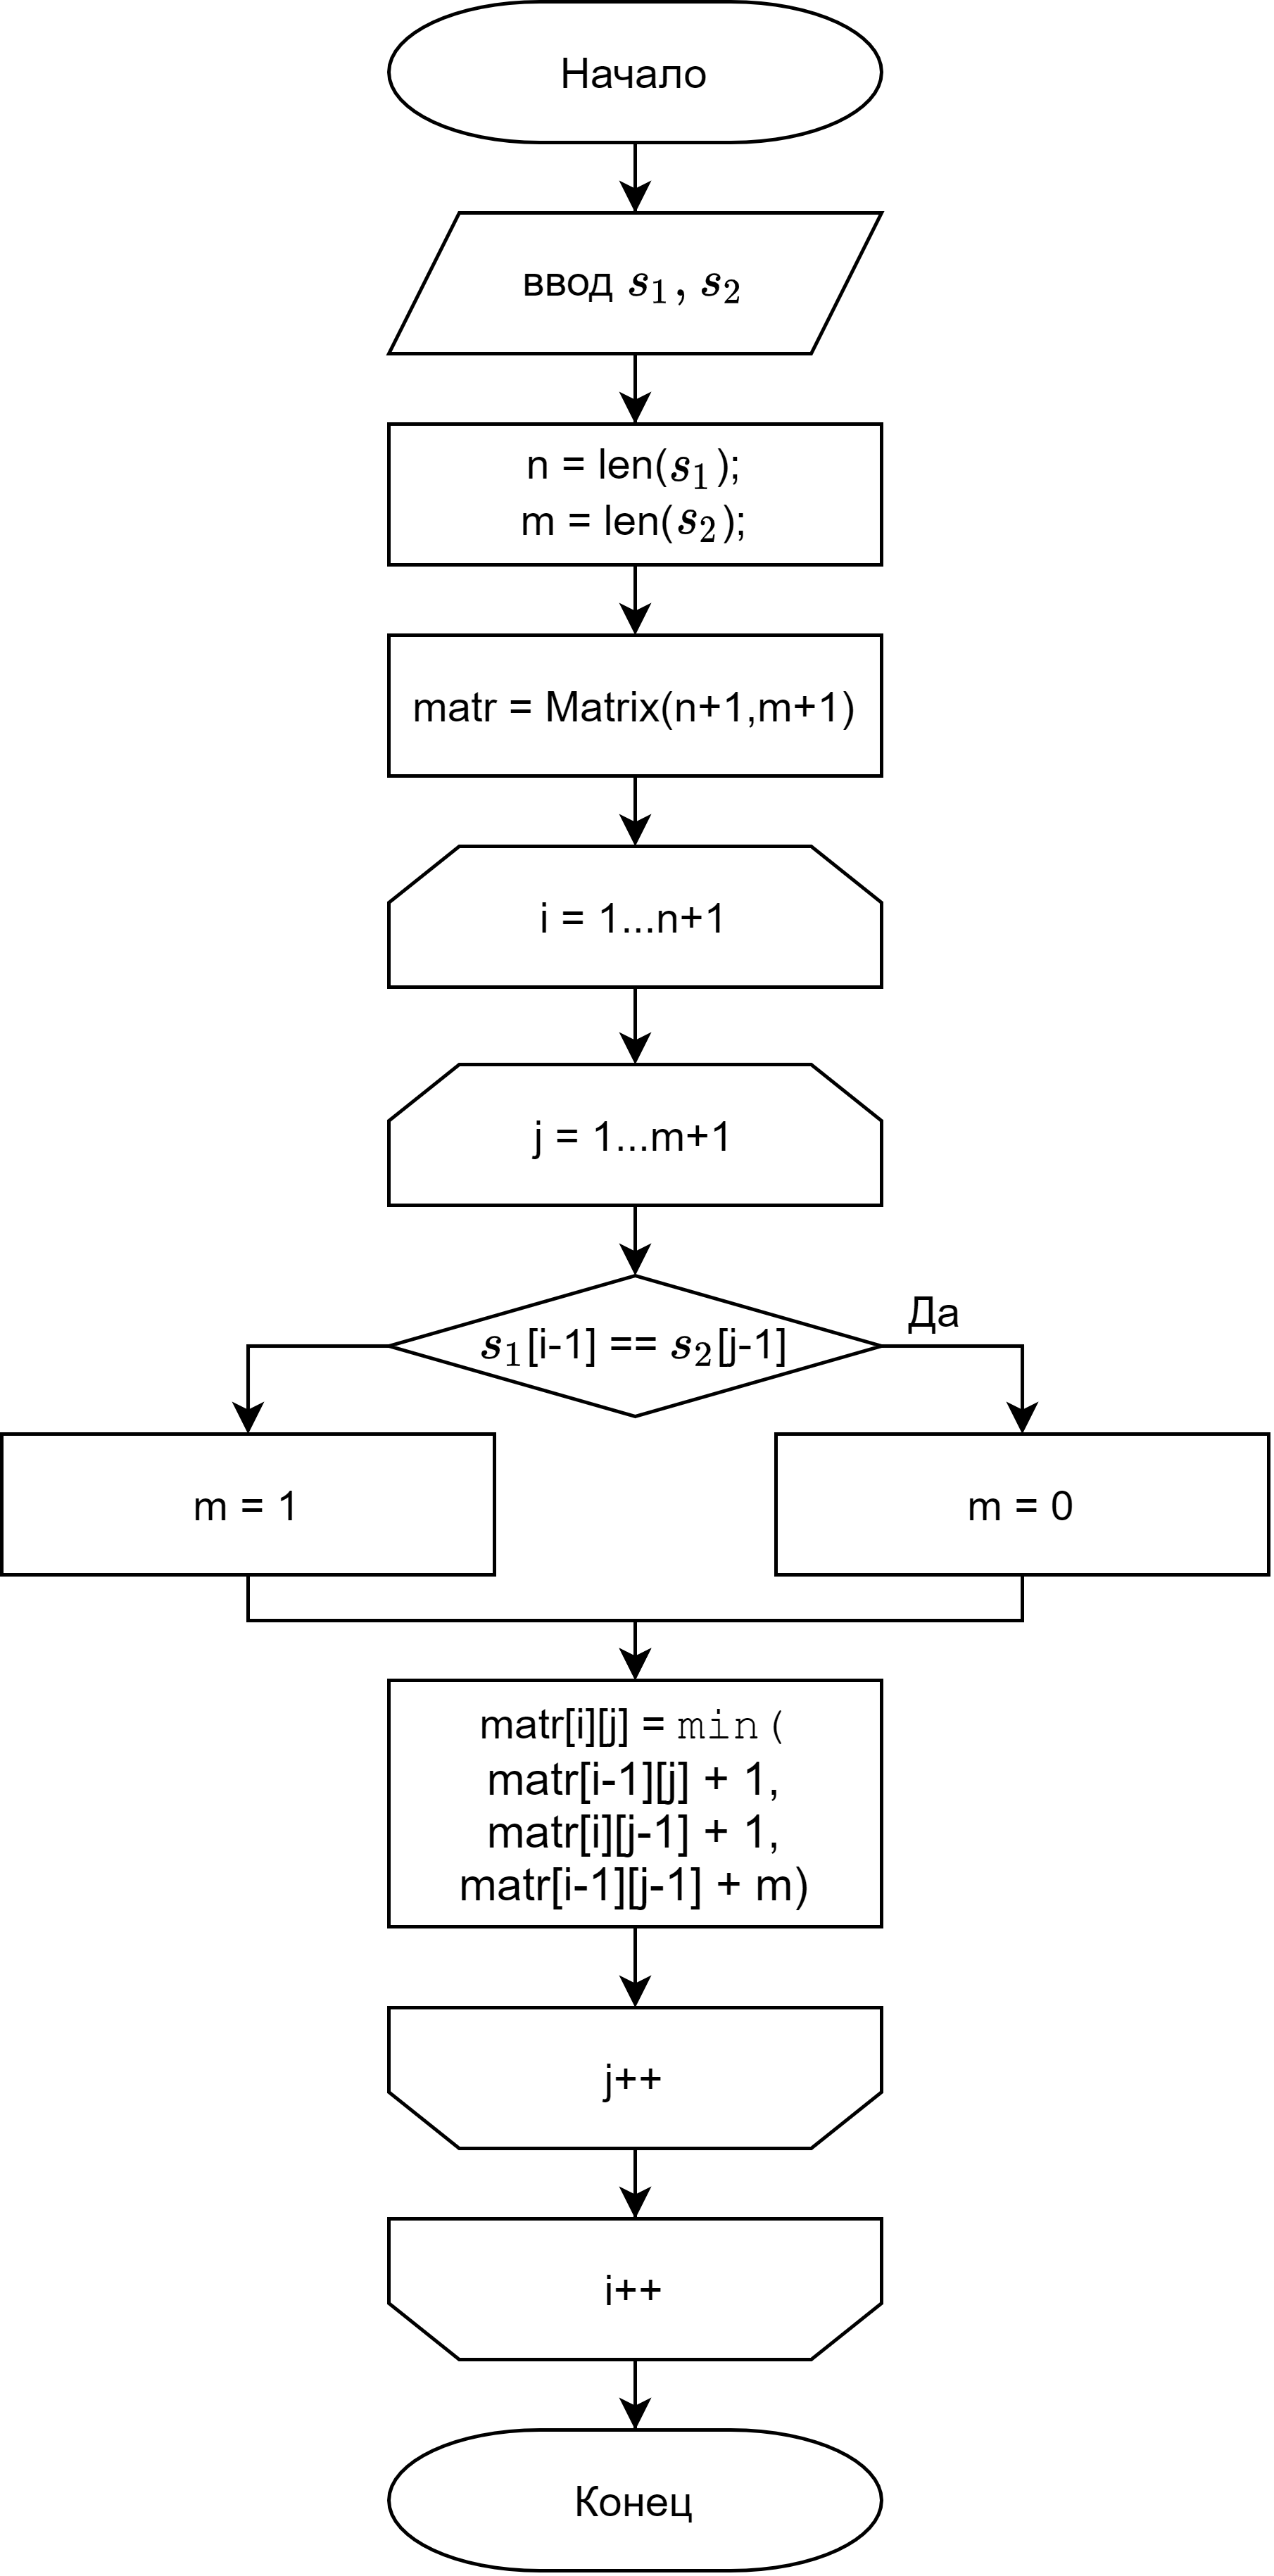
\includegraphics[scale=0.18]{LevMatr}
        \caption{Схема нерекурсивного поиска с заполнением матрицы}
        \label{schema:matr:Levenstein}
    \end{figure}

    \begin{figure}[h!]
        \centering
        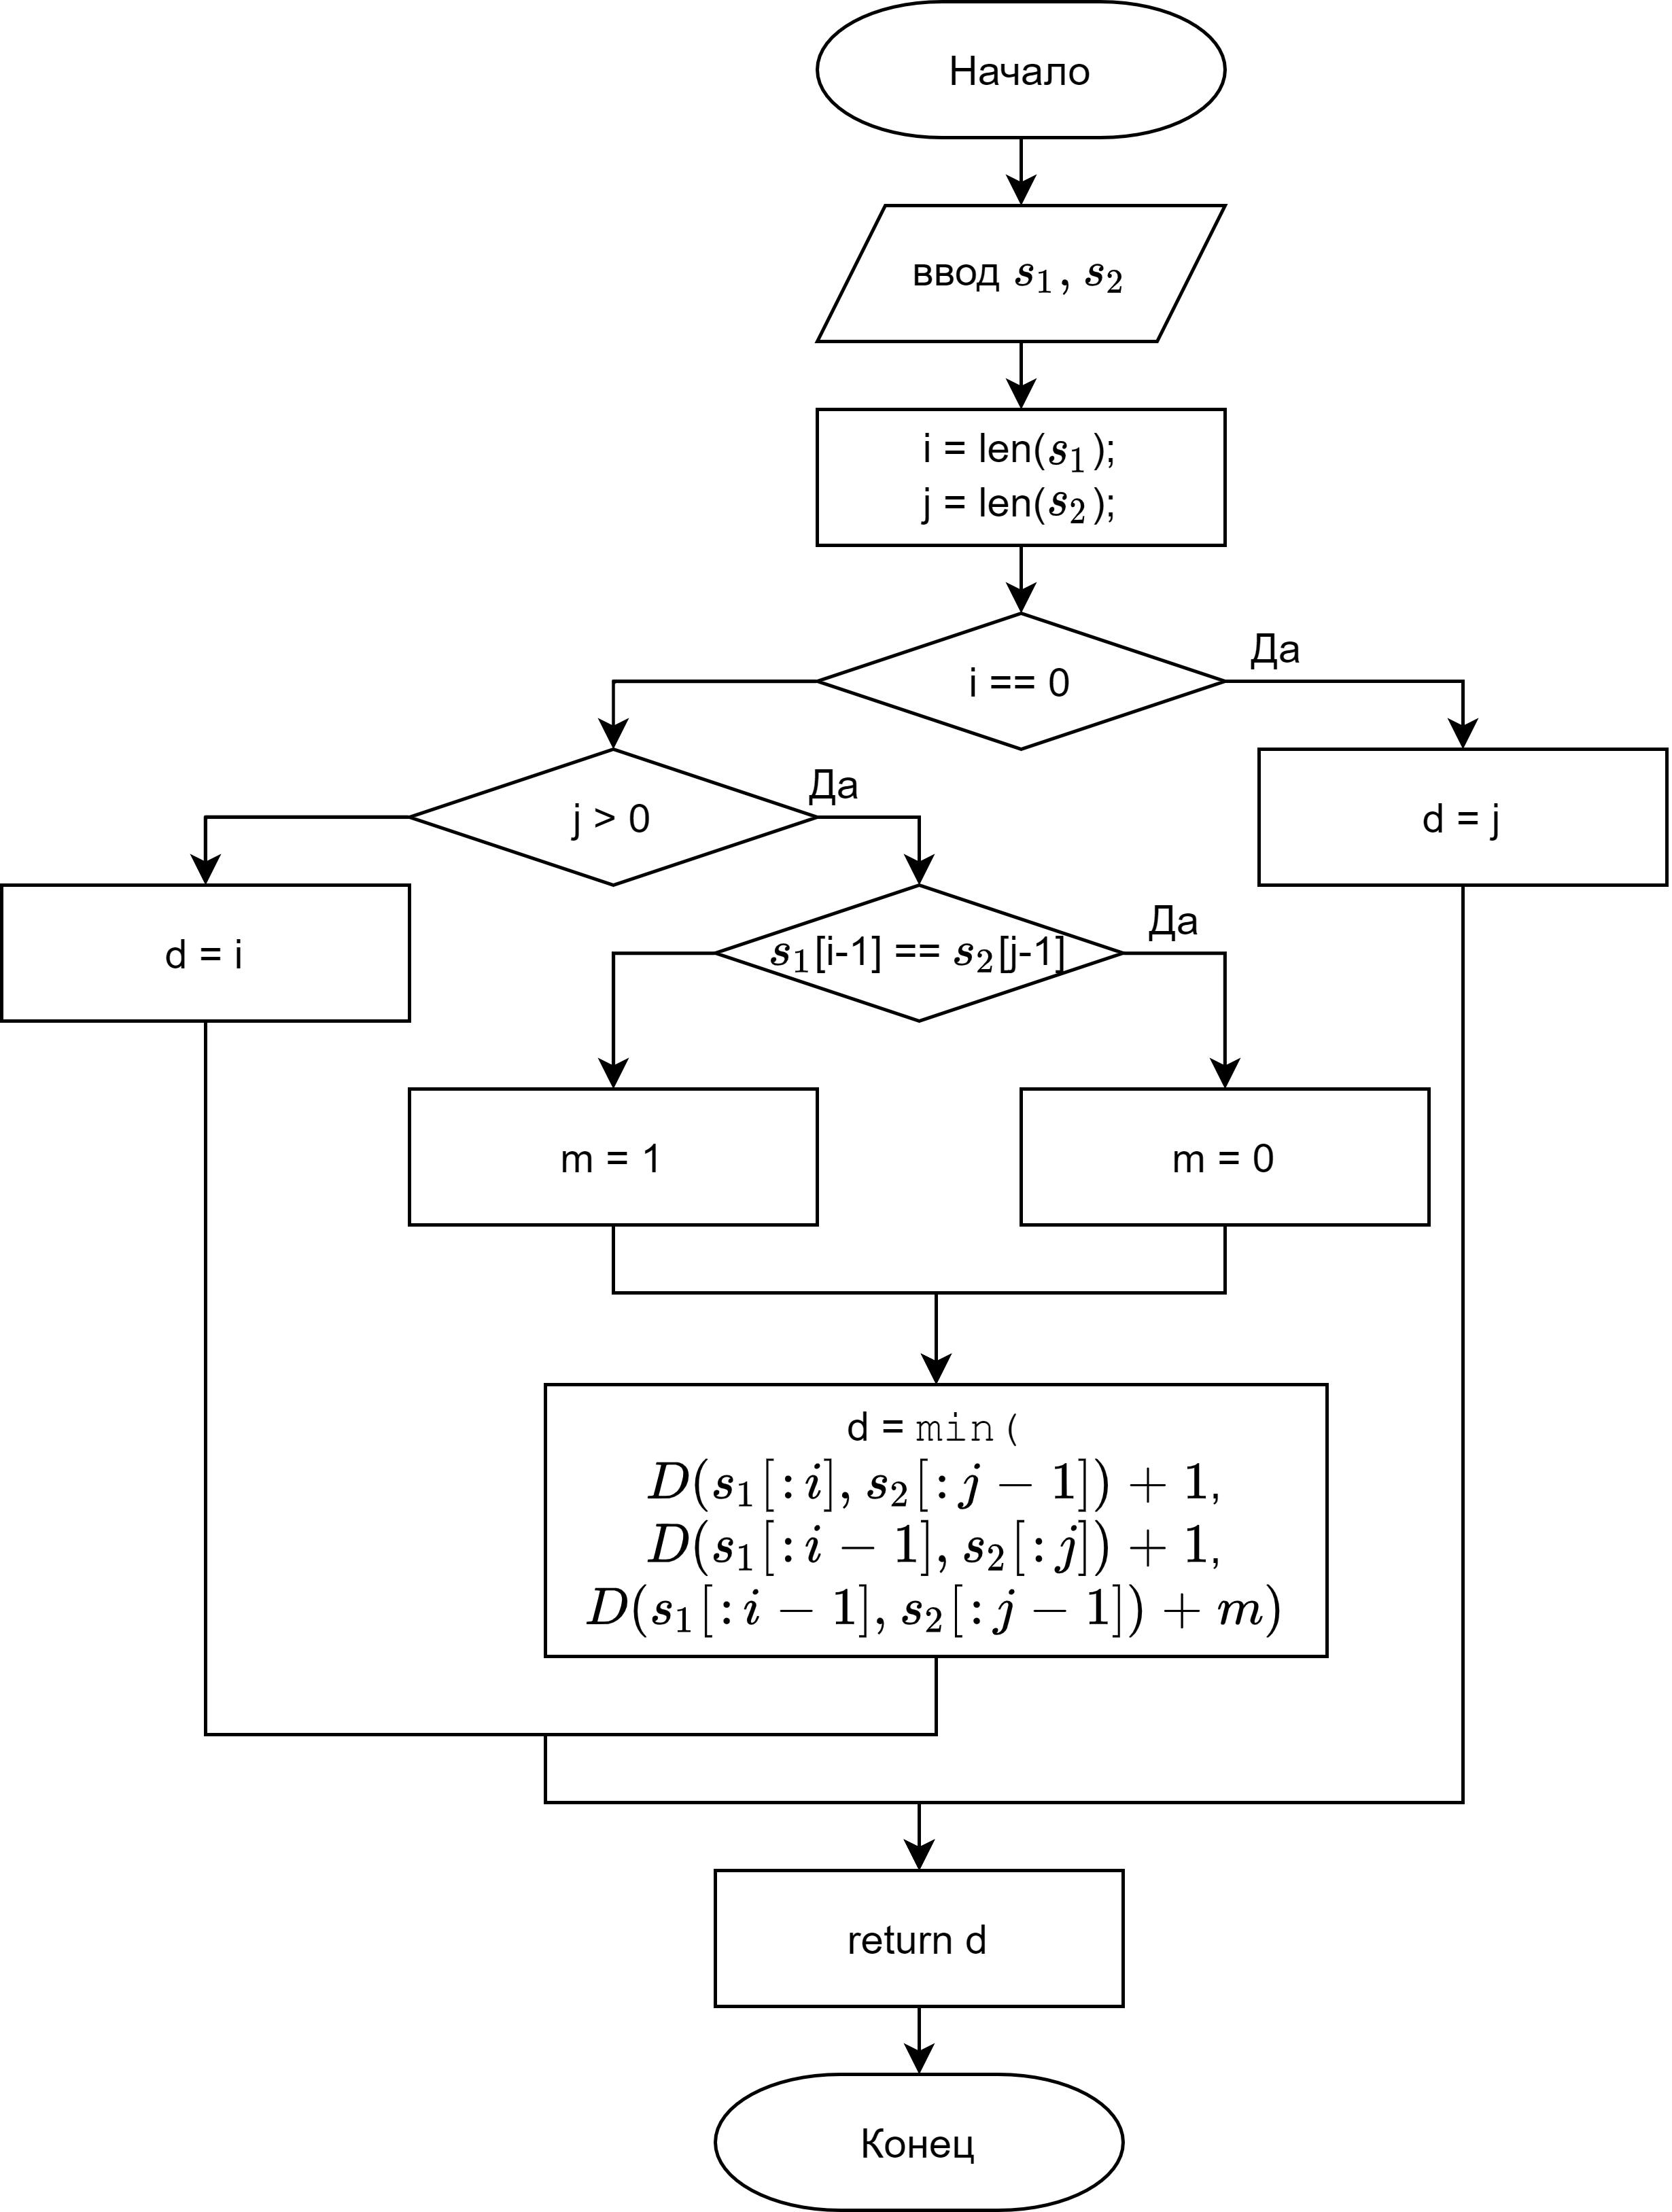
\includegraphics[scale=0.18]{LevRec}
        \caption{Схема рекурсивого поиска без заполнения матрицы}
        \label{schema:rec:Levenstein}
    \end{figure}

    \begin{figure}[h!]
        \centering
        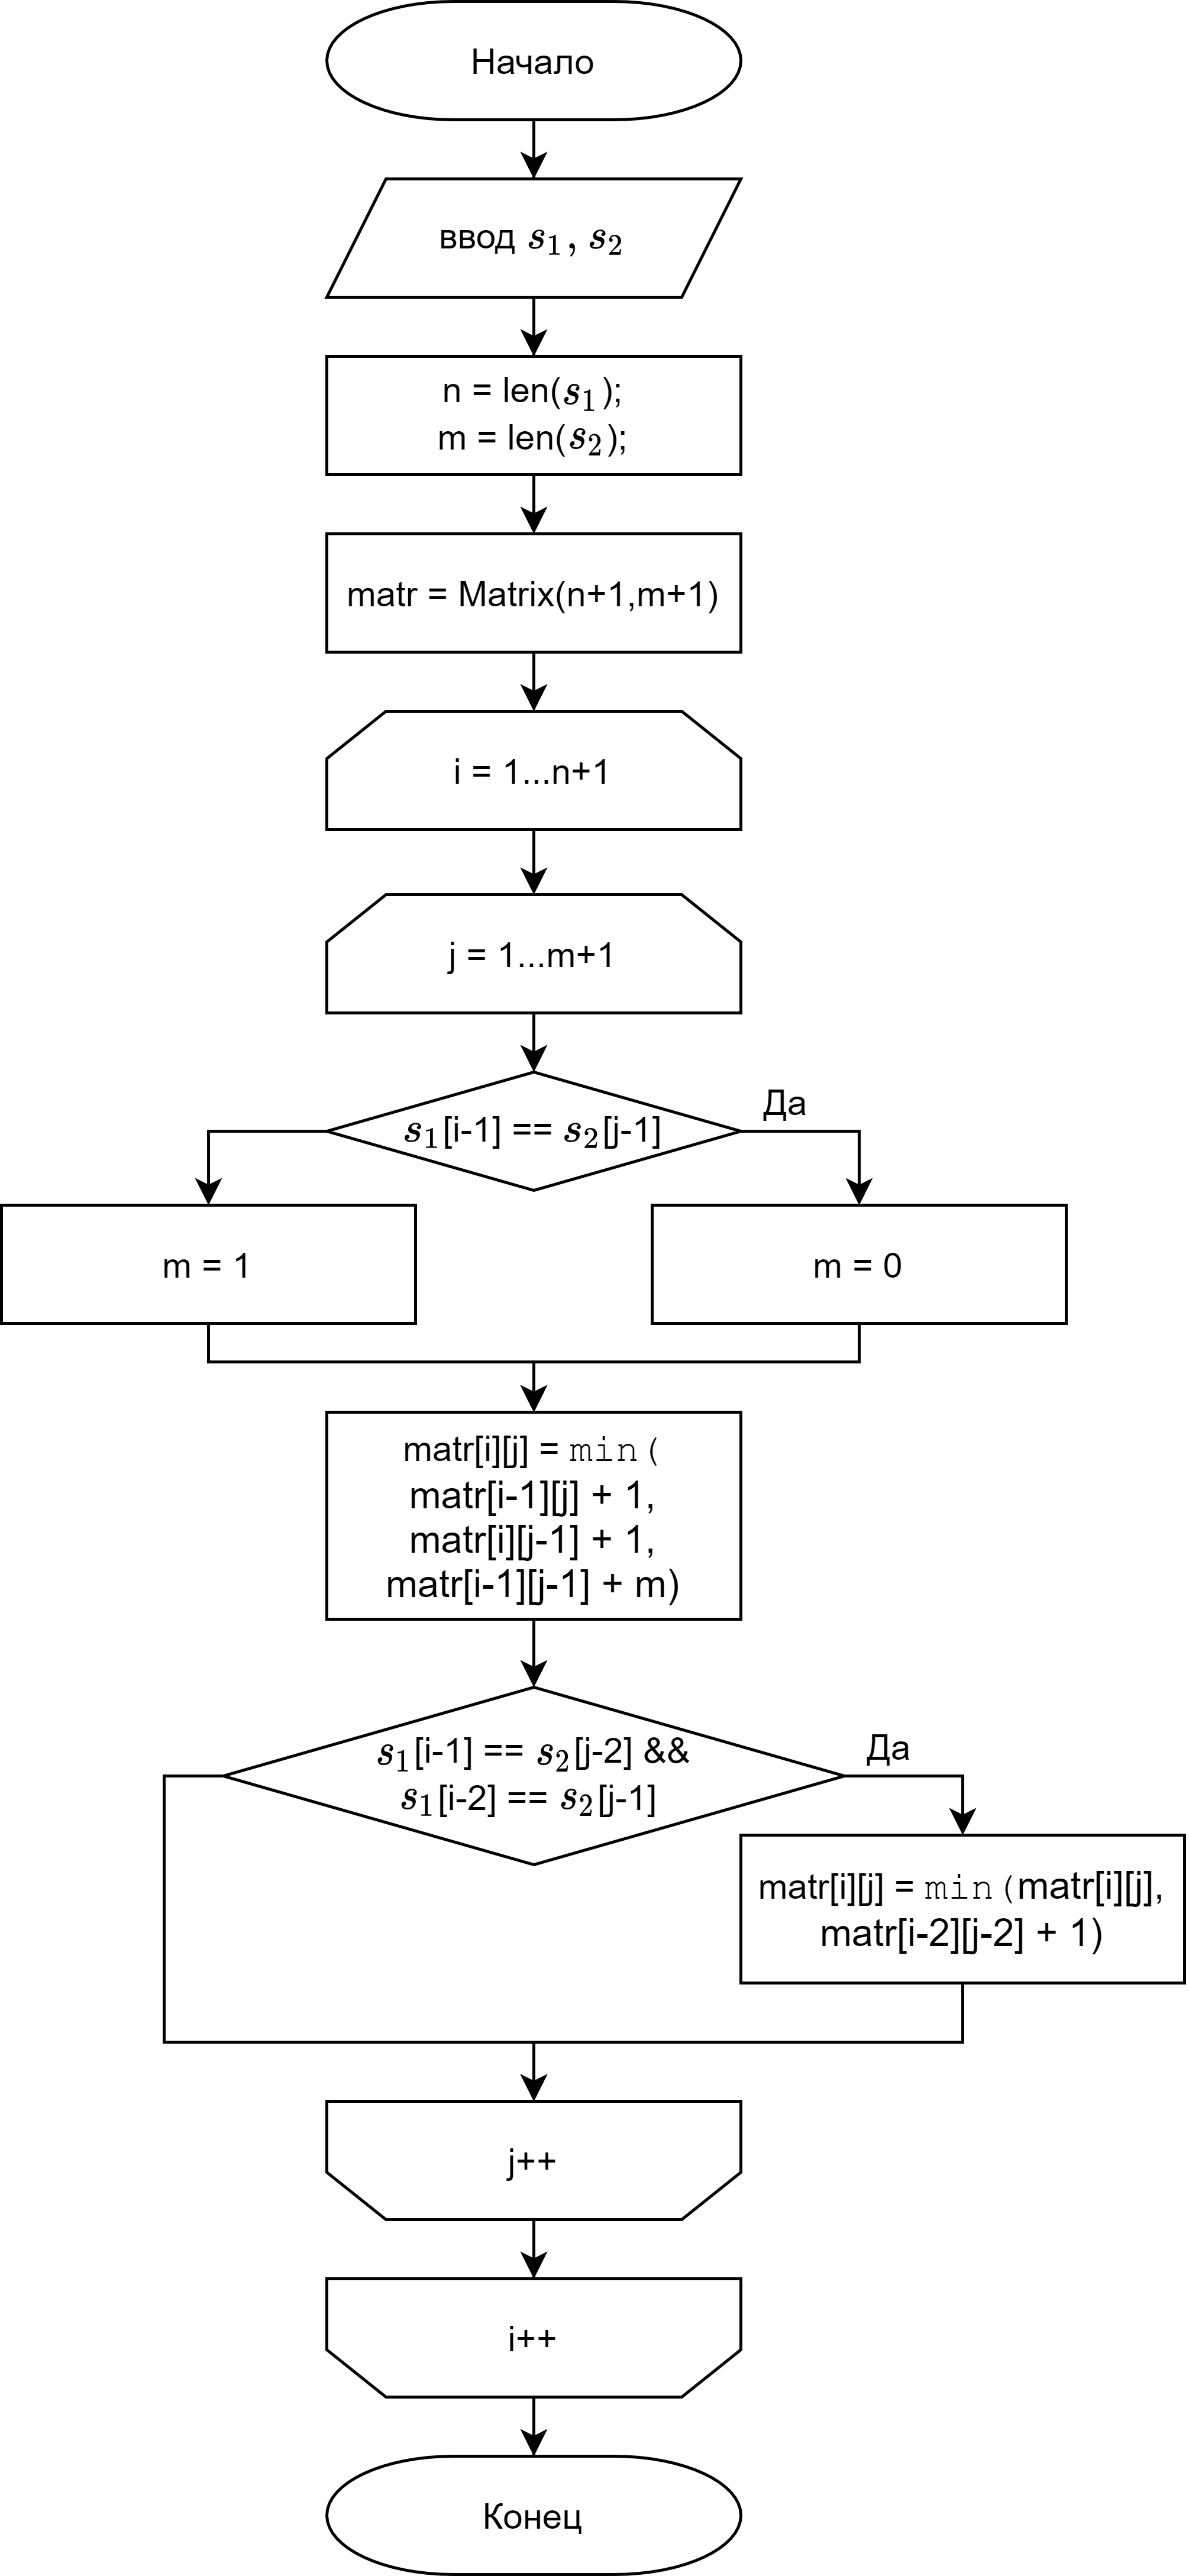
\includegraphics[scale=0.16]{DamLevMatr}
        \caption{Схема рекурсивого поиска с заполнением матрицы}
        \label{schema:rec-matr:Levenstein}
    \end{figure}

    \begin{figure}[h!]
        \centering
        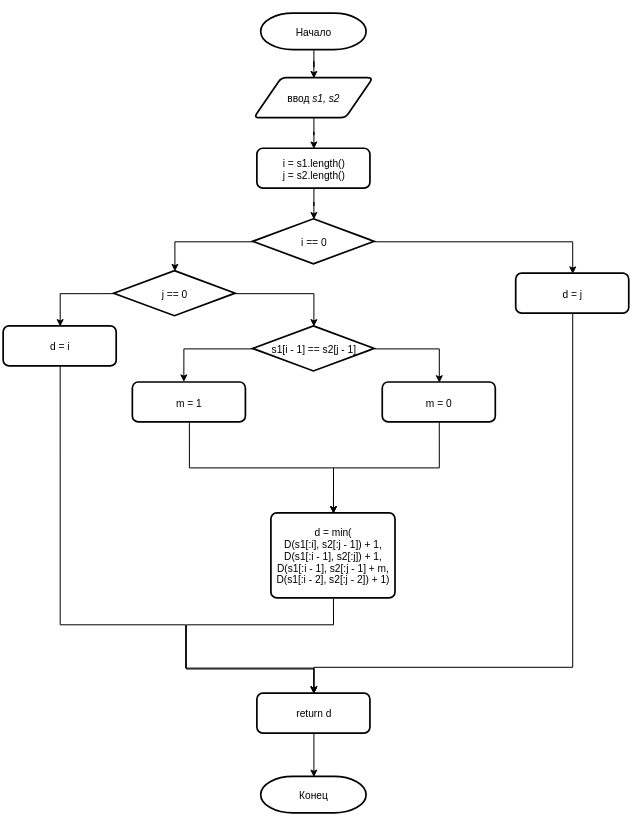
\includegraphics[scale=1]{LevGraph}
        \caption{Схема поиска р. Дамерау-Левенштейна}
        \label{schema:matr:Dameray-Levenstein}
    \end{figure}

\newpage
\chapter{ Технологический раздел}
\label{cha:technological}

    В данном разделе будут выбраны средства реплизации ПО, представлен листинг кода
    и проведён теоритический анализ максимальной затрачиваемой памяти. 

    \section{Средства реализации}
        В данной работе используется язык программирования python \cite{python}, так как
        он позволяет написать программу в относительно малый срок.
        В качестве среды разработки использовалась Visual Studio Code \cite{visual-studio-code}.

        Для замера процессорного времени была использована функция process\_time \cite{process_time} модуля time.
        Она возвращает значение в долях секунды суммы системного и пользовательского процессорного времени текущего процесса и 
        не включает время, прошедшее во время сна.

    \section{Листинг программы}
        Ниже представлены листинги кода умножения матриц:
        \begin{enumerate}
            \item стандартной реализации (листинг \ref{lst:standartDot});
            \item реализация алгоритма Винограда (листинг \ref{lst:vinogradDot});
            \item реализация оптимизированного алгоритма Винограда (листинг \ref{lst:vinogradDot:optimize}).
        \end{enumerate}
        
        \begin{lstlisting}[language=python, label=lst:standartDot, caption=Реализация классического алгоритма умножения матриц]
def dotMatrix(matr_a : list, matr_b: list) -> (list, float):
    if (len(matr_b) != len(matr_a[0])):
        raise ValueError
    
    m = len(matr_a)
    n = len(matr_a[0])
    q = len(matr_b[0])
    matr_c = [[0] * q for i in range(m)]

    t_start = process_time()
    for i in range(m):
        for j in range(q):
            for k in range(n):
                matr_c[i][j] = matr_c[i][j] + matr_a[i][k] * matr_b[k][j]
    t_end = process_time()

    return matr_c, t_end - t_start
        \end{lstlisting}

        \begin{lstlisting}[language=python, label=lst:vinogradDot, caption=Реализация алгоритма Винограда умножения матриц]
def dotMatrixVinograd(matr_a : list, matr_b: list) -> (list, float):
    if (len(matr_b) != len(matr_a[0])):
        raise ValueError
    
    m = len(matr_a)
    n = len(matr_a[0])

    q = len(matr_b[0])
    matr_c = [[0] * q for i in range(m)]

    row = [0] * m
    col = [0] * q

    t_start = process_time()

    for i in range(m):
        for j in range(n // 2):
            row[i] = row[i] + matr_a[i][2*j] * matr_a[i][2*j + 1]
    
    for j in range(q):
        for i in range(n // 2):
            col[j] = col[j] + matr_b[2*i][j] * matr_b[2*i+1][j]

    for i in range(m):
        for j in range(q):
            matr_c[i][j] = -row[i] - col[j]
            for k in range(n//2):
                matr_c[i][j] = matr_c[i][j] + (matr_a[i][2*k+1] + matr_b[2*k][j]) * (matr_a[i][2*k] + matr_b[2*k+1][j])

    if n % 2:
        for i in range(m):
            for j in range(q):
                matr_c[i][j] = matr_c[i][j] + matr_a[i][n-1] * matr_b[n-1][j]
    t_end = process_time()

    return matr_c, t_end - t_start
        \end{lstlisting}

        \begin{lstlisting}[language=python, label=lst:vinogradDot:optimize, caption=Реализация оптимизированного алгоритма Винограда умножения матриц]
def dotMatrixVinogradOptimizate(matr_a : list, matr_b: list) -> (list, float):
    if (len(matr_b) != len(matr_a[0])):
        raise ValueError
    
    m = len(matr_a)
    n = len(matr_a[0])
    q = len(matr_b[0])
    matr_c = [[0] * q for i in range(m)]

    row = [0] * m
    col = [0] * q
    t_start = process_time()
    for i in range(m):
        for j in range(1, n, 2):
            row[i] -= matr_a[i][j] * matr_a[i][j - 1]
    
    for j in range(q):
        for i in range(1, n, 2):
            col[j] -= matr_b[i][j] * matr_b[i - 1][j]

    for i in range(m):
        for j in range(q):
            matr_c[i][j] = row[i] + col[j]
            for k in range(1, n, 2):
                matr_c[i][j] += (matr_a[i][k - 1] + matr_b[k][j]) * (matr_a[i][k] + matr_b[k-1][j])

    if n % 2:
        for i in range(m):
            for j in range(q):
                matr_c[i][j] += matr_a[i][n-1] * matr_b[n-1][j]
    t_end = process_time()

    return matr_c, t_end - t_start
        \end{lstlisting}
    
        
    \section{Тестирование}
        В таблице \ref{table:testing} отображён возможный набор тестов
        для тестирования методом чёрного ящика, результаты которого, 
        представленные на рисунке \ref{png:testing:result}, подтверждают
        прохождение программы перечисленных тестов.

        \begin{table}[]
            \caption{Тесты для проверки корректности программы}

            \centering
            \begin{tabular}{|c|c|c|}
                \hline
                Матрица A                                                & Матрица B                                              & Ожидаемый результат                                    \\ \hline
                $\begin{bmatrix} 0 & 0 \\ 0 & 0 \end{bmatrix}$           & $\begin{bmatrix} 1 & 1 & 1 \\ 1 & 1 & 1 \end{bmatrix}$ & $\begin{bmatrix} 0 & 0 & 0 \\ 0 & 0 & 0 \end{bmatrix}$ \\ \hline
                $\begin{bmatrix} 1 & 0 \\ 0 & 1 \end{bmatrix}$           & $\begin{bmatrix} 1 & 1 & 1 \\ 1 & 1 & 1 \end{bmatrix}$ & $\begin{bmatrix} 1 & 1 & 1 \\ 1 & 1 & 1 \end{bmatrix}$ \\ \hline
                $\begin{bmatrix} 1 & 1 \\ 1 & 1 \\ 1 & 1 \end{bmatrix}$  & $\begin{bmatrix} 1 & 1 & 1 \\ 1 & 1 & 1 \end{bmatrix}$ & $\begin{bmatrix} 2 & 2 & 2 \\ 2 & 2 & 2 \\ 2 & 2 & 2 \end{bmatrix}$ \\ \hline
                $\begin{bmatrix} 1 \\ 1 \end{bmatrix}$                   & $\begin{bmatrix} 1 & 1 & 1 \\ 1 & 1 & 1 \end{bmatrix}$ & the matrices cannot be multiplied                       \\ \hline
                \end{tabular}
            \label{table:testing}
        \end{table}
        
        \begin{figure}[h!]
            \centering
            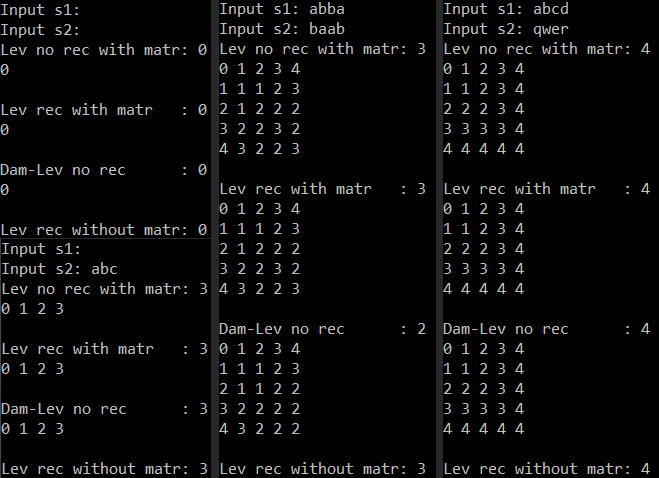
\includegraphics[scale=0.9]{testing.png}
            \caption{Результаты тестирования алгоритмов: стандартного, Винограда и оптимизированного Винограда}
            \label{png:testing:result}
        \end{figure}
\newpage
\chapter{Экспериментальный раздел}
\label{cha:research}
    В данном разделе будут проведены эксперименты для проведения 
    сравнительного анализа алгоритмов по затрачиваемому процессорному 
    времени и максимальной используемой памяти.
% и количеству максимально затрачиваемой памяти
    \section{Сравнительный анализ на основе замеров времени работы алгоритмов}
        В рамках данного проекта были проведёны следующие эксперименты:

        1) сравнение алгоритмов поиска расстояния Левенштейна и Дамерау-Левенштейна
        на строках длиной от 0 до 5 с шагом 1 (рисунок \ref{png:test:1});
        
        2) сравнение алгоритмов \footnote{Замеры времени для рекурсивного алгоритма поиска расстояния Левенштейна
        на строках длиной от 0 до 975 с шагом 75 не проводились, так как уже на
        строках длиной 10 алгоритм работает 70 034 ms, что в 35 000 раз больше, 
        времени работы алгоритмов с использованием матрицы. Это связано с экспоненциальной асимптотикой
        времени выполнения данного алгоритма (пропорционально количеству
        рекурсивных вызовов).} поиска расстояния Левенштейна и Дамерау-Левенштейна
        на строках длиной от 0 до 1000 с шагом 50 (рисунок \ref{png:test:2}).
        
        Тестирование проводилось на стационаном компьютере с процессором
        Intel(R) Core(TM) i5-7200U CPU 2.50 GHz
        под управлением Debian 10 с 8 Гб оперативной памяти.

        Ниже предствалены графики зависимости времени работы алгоритмов от длины входных строк
        (рисунки \ref{graph:test:1} и \ref{graph:test:2}).

        \begin{figure}[h!]
            \centering
            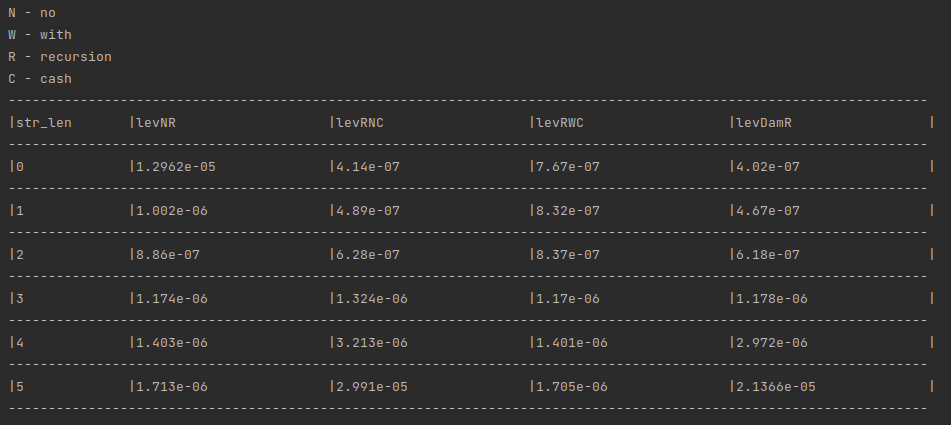
\includegraphics[scale=0.7]{TimeTable5Elems.png}
            \caption{Результаты замера времени на строках длиной от 0 до 5}
            \label{png:test:1}
        
            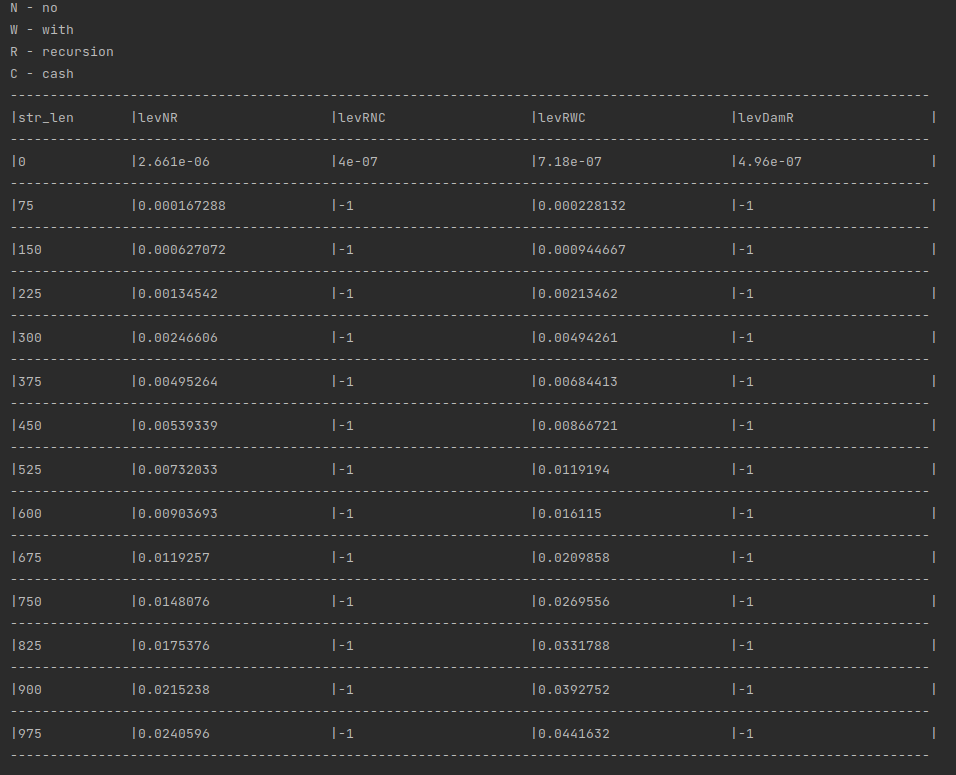
\includegraphics[scale=0.7]{TimeTable975Elems.png}
            \caption{Результаты замера времени на строках длиной от 0 до 975}
            \label{png:test:2}
        \end{figure}

        \begin{figure}[h!]
            \centering
            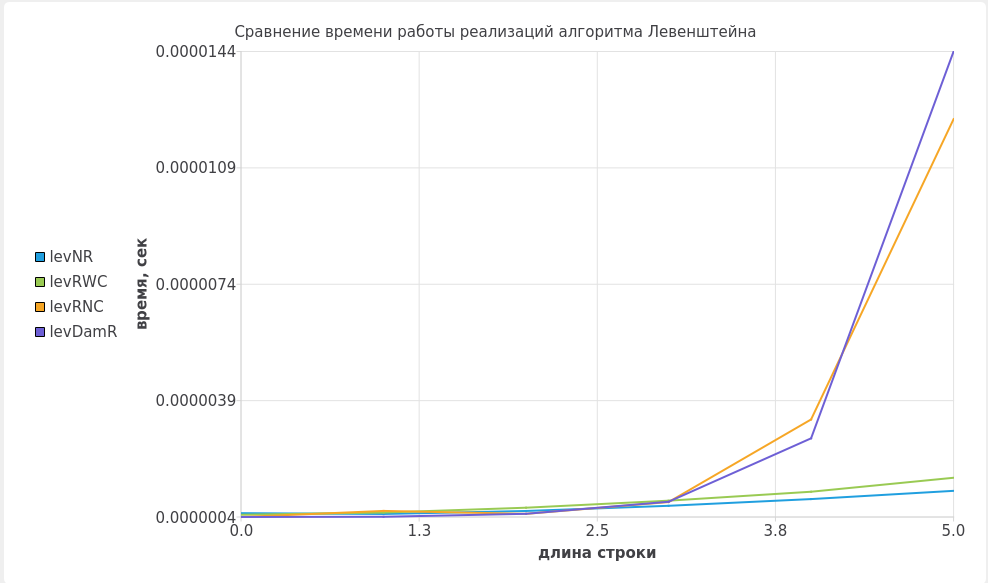
\includegraphics[scale=0.7]{smallGraphic.png}
            \caption{График зависимости времени работы алгоритмов от длин строк}
            \label{graph:test:1}

            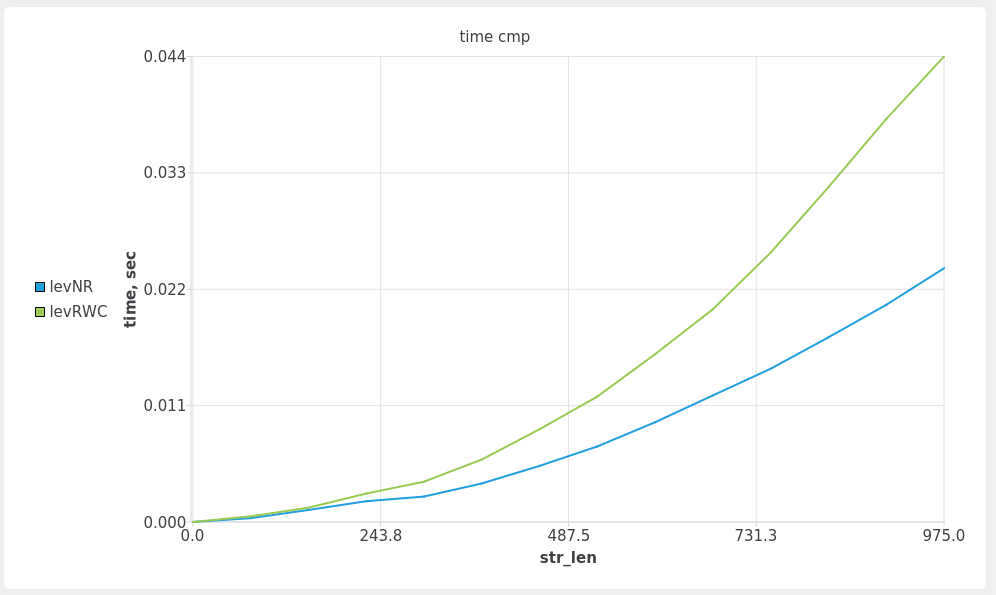
\includegraphics[scale=0.7]{LargeGraphic.png}
            \caption{График зависимости времени работы алгоритмов от длин строк}
            \label{graph:test:2}
        \end{figure}

    \section{Вывод}
        В данном разделе были поставлены эксперименты по замеру времени
        выполнения каждого из алгоритмов. По итогам замеров не рекурсивный 
        алгоритм нахождения расстояния Левенштейна оказался самым быстродействующим
        на длинах строк превышающих 3 на 136 \% быстрее, чем алгоритм поиска
        расстояния Левенштейна рекурсивно с заполнением матрицы и на 42 \%,
        чем реализация алгоритм поиска расстояния Дамерау-Левенштейна. На строках
        длиной менее 3х символов рекурсивная реализиция выигрывает матричные, так
        как не выделяет в куче место под хранение матрицы.  
        
        По расходу памяти матричные алгоритмы проигрывают рекурсивному, так как
        максимальный размер используемой памяти имеет квадратичную ассимптотику
        (произведение длин строк), в то время как у рекурсивного - линейная (сумма длин строк).


\newpage

\backmatter % Здесь заканчивается нумерованная часть документа и начинаются ссылки и
\Conclusion
    В ходе работы были изучены и реализованы алгоритмы нахождения
    расстояния Левенштейна (не рекурсивный с заполнением матрицы,
    рекурсивный без заполнения матрицы, рекурсивный с заполнением матрицы)
    и Дамерау-Левенштейна (не рекурсивный с заполнением матрицы). 
    Выполнено сравнение перечисленных алгоритмов. 
    
    В ходе экспериментов по замеру времени работы было установлено, что не рекурсивный алгоритм нахождения расстояния Левенштейна
    на длинах строк превышающих 3 на 136 \% быстрее, чем алгоритм поиска
    расстояния Левенштейна рекурсивно с заполнением матрицы и на 42 \%,
    чем реализация алгоритм поиска расстояния Дамерау-Левенштейна. На строках
    длиной менее 3 символов рекурсивная реализиция работает бысрее матричной, так
    как не выделяет в куче место под хранение матрицы.
    
    Из теоритического анализа максимальной затрачиваемой памяти каждым из алгоритмов 
    представленым в технологической части можно сделать вывод, что реализации
    с использованием матриц занимают намного больше памяти при обработке
    длинных строк, чем рекурсивная реализация, так при длине строк 1000
    символов, рекурсивный алгоритм теоритически использует в 95.5 раз меньше памяти, чем остальные.

% % Список литературы при помощи BibTeX
% Юзать так:
%
% pdflatex report
% bibtex report
% pdflatex report

\bibliographystyle{gost780u}
\bibliography{report}

\end{document}